\documentclass[tikz,border=3.14mm]{standalone}
\usetikzlibrary{shapes.geometric,positioning,arrows.meta,fit,shadows}

\makeatletter
\pgfkeys{/pgf/.cd,
  parallelepiped offset x/.initial=2mm,
  parallelepiped offset y/.initial=2mm
}

\pgfdeclareshape{parallelepiped}{
  \inheritsavedanchors[from=rectangle] % this is nearly a rectangle
  \inheritanchorborder[from=rectangle]
  \inheritanchor[from=rectangle]{north}
  \inheritanchor[from=rectangle]{north west}
  \inheritanchor[from=rectangle]{north east}
  \inheritanchor[from=rectangle]{center}
  \inheritanchor[from=rectangle]{west}
  \inheritanchor[from=rectangle]{east}
  \inheritanchor[from=rectangle]{mid}
  \inheritanchor[from=rectangle]{mid west}
  \inheritanchor[from=rectangle]{mid east}
  \inheritanchor[from=rectangle]{base}
  \inheritanchor[from=rectangle]{base west}
  \inheritanchor[from=rectangle]{base east}
  \inheritanchor[from=rectangle]{south}
  \inheritanchor[from=rectangle]{south west}
  \inheritanchor[from=rectangle]{south east}
  \backgroundpath{
    % Define the path for the shape
    \southwest \pgf@xa=\pgf@x \pgf@ya=\pgf@y
    \northeast \pgf@xb=\pgf@x \pgf@yb=\pgf@y
    \pgfmathsetlength\pgfutil@tempdima{\pgfkeysvalueof{/pgf/parallelepiped offset x}}
    \pgfmathsetlength\pgfutil@tempdimb{\pgfkeysvalueof{/pgf/parallelepiped offset y}}
    \def\ppd@offset{\pgfpoint{\pgfutil@tempdima}{\pgfutil@tempdimb}}
    \pgfpathmoveto{\pgfqpoint{\pgf@xa}{\pgf@ya}}
    \pgfpathlineto{\pgfqpoint{\pgf@xb}{\pgf@ya}}
    \pgfpathlineto{\pgfqpoint{\pgf@xb}{\pgf@yb}}
    \pgfpathlineto{\pgfqpoint{\pgf@xa}{\pgf@yb}}
    \pgfpathclose
    \pgfpathmoveto{\pgfqpoint{\pgf@xb}{\pgf@ya}}
    \pgfpathlineto{\pgfpointadd{\pgfpoint{\pgf@xb}{\pgf@ya}}{\ppd@offset}}
    \pgfpathlineto{\pgfpointadd{\pgfpoint{\pgf@xb}{\pgf@yb}}{\ppd@offset}}
    \pgfpathlineto{\pgfpointadd{\pgfpoint{\pgf@xa}{\pgf@yb}}{\ppd@offset}}
    \pgfpathlineto{\pgfqpoint{\pgf@xa}{\pgf@yb}}
    \pgfpathmoveto{\pgfqpoint{\pgf@xb}{\pgf@yb}}
    \pgfpathlineto{\pgfpointadd{\pgfpoint{\pgf@xb}{\pgf@yb}}{\ppd@offset}}
  }
}

\begin{document}
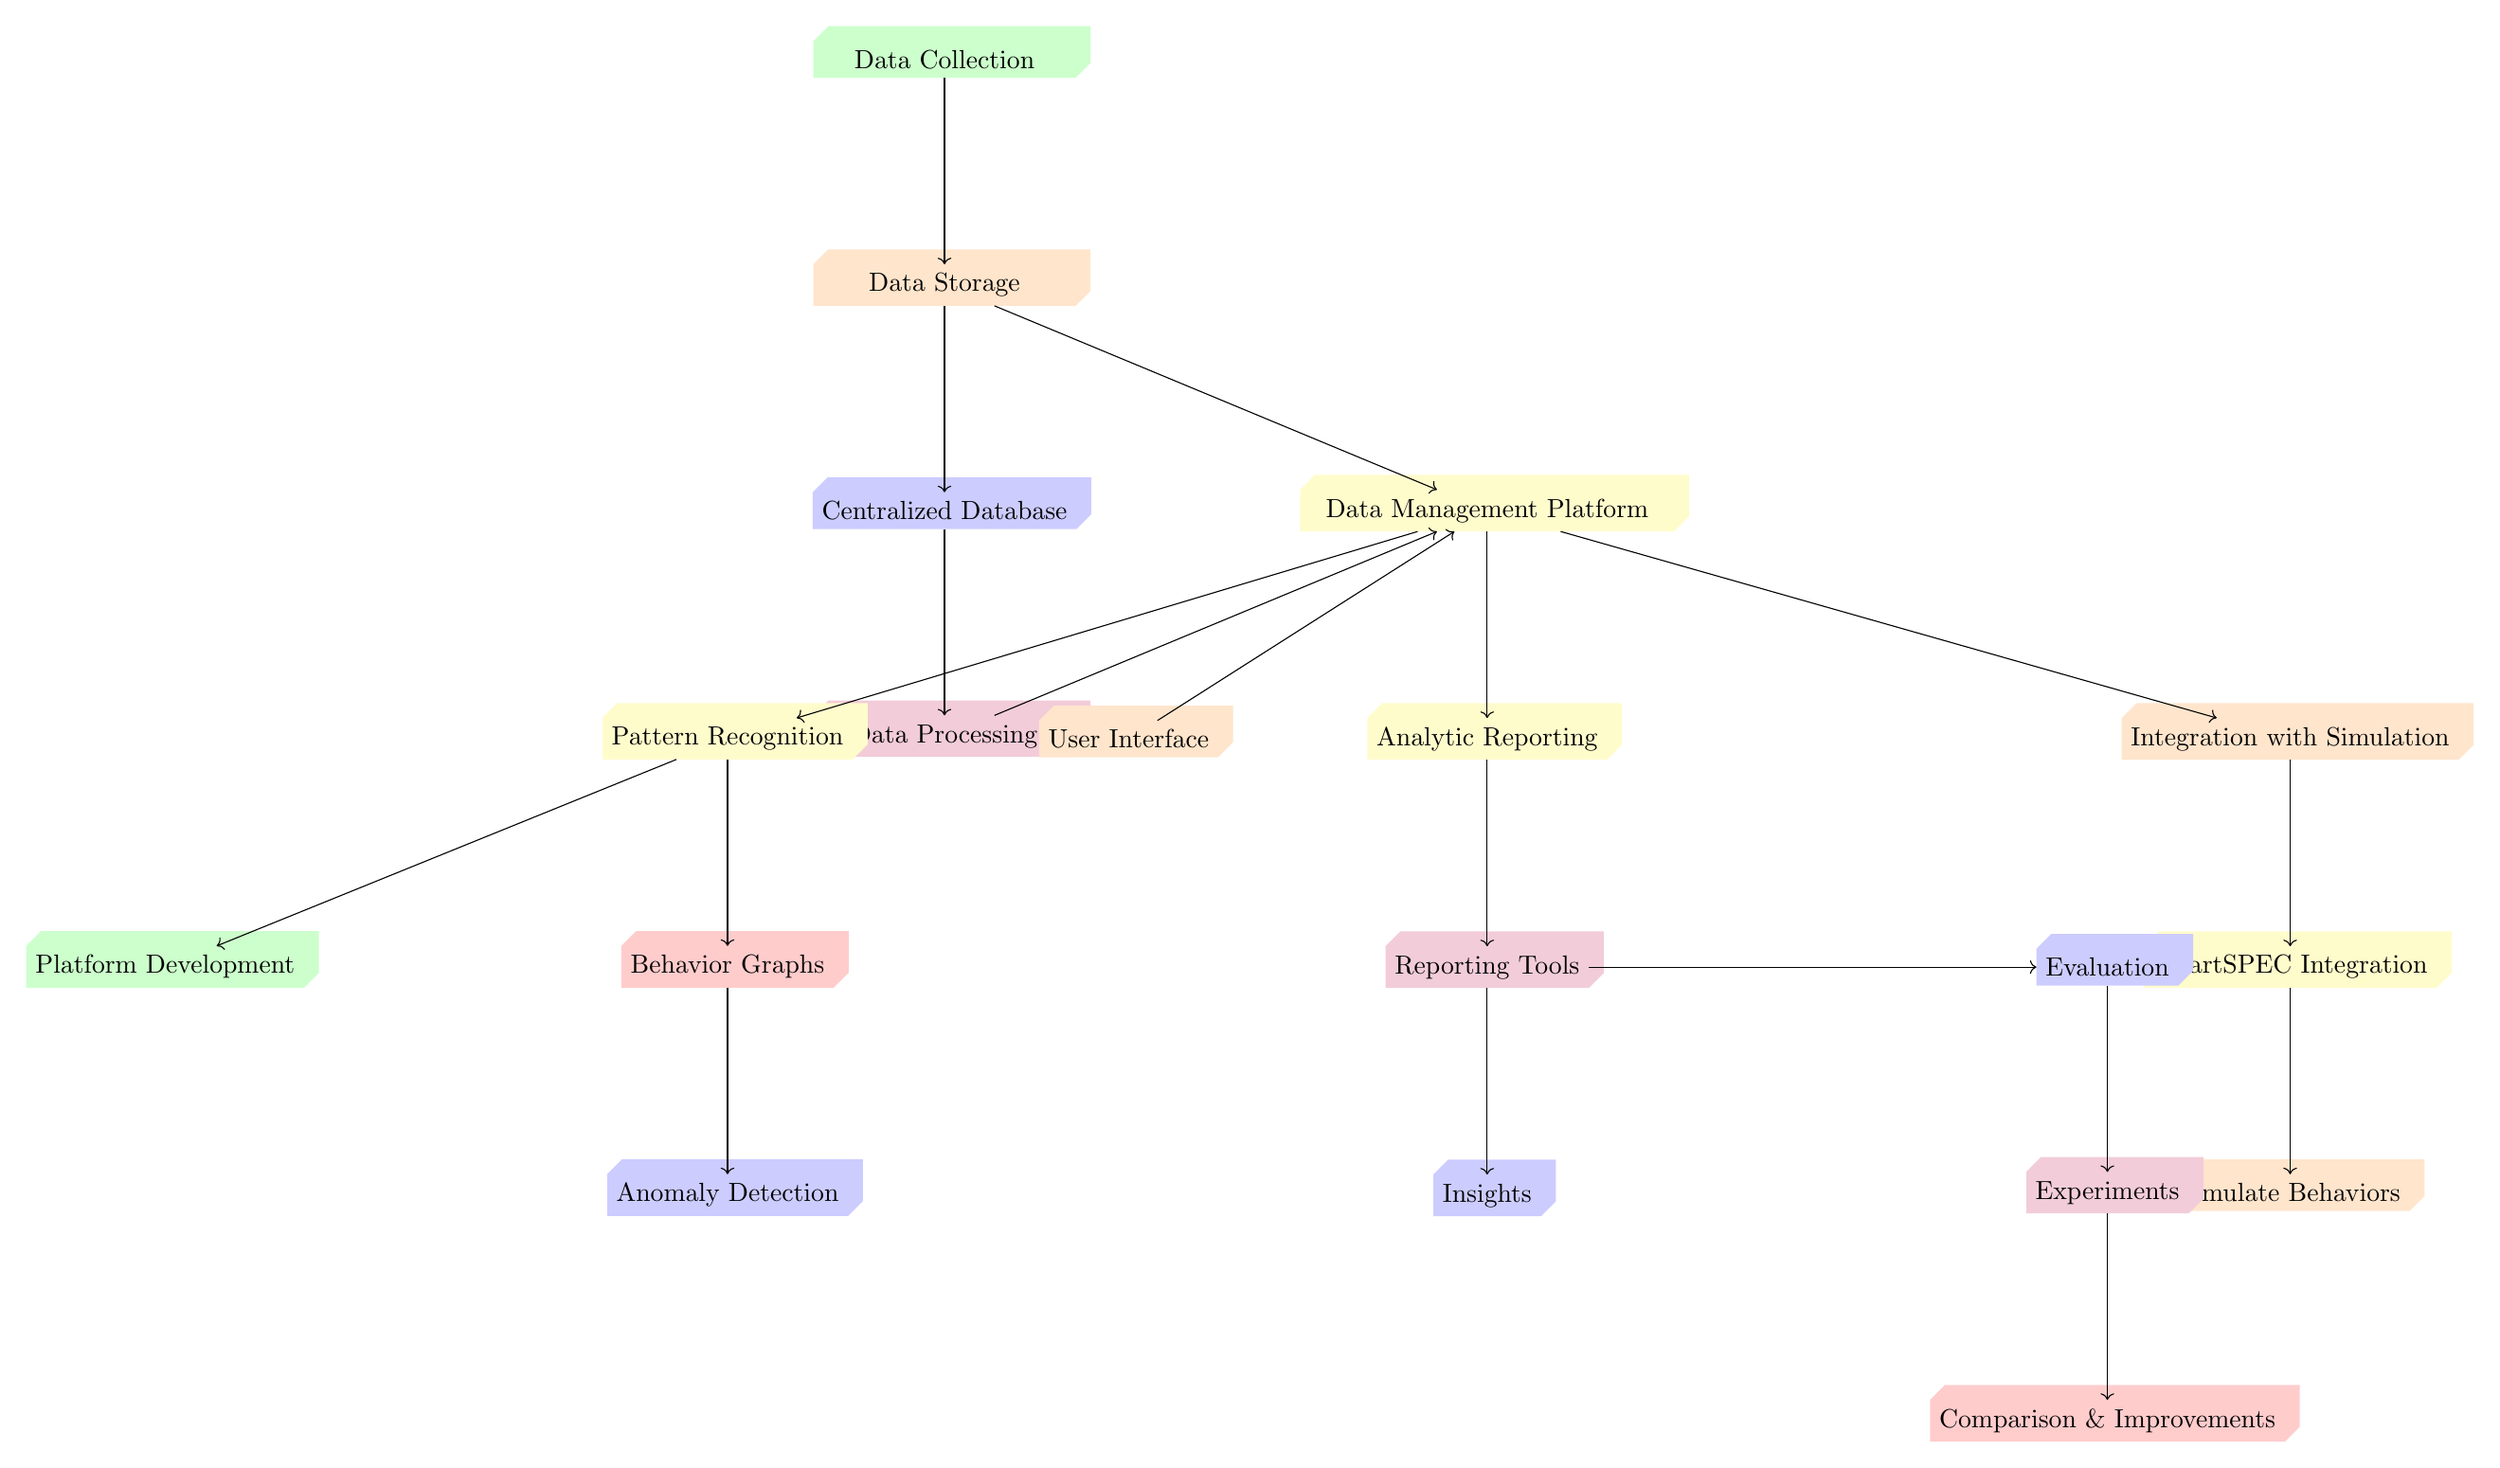
\begin{tikzpicture}[node distance=2.5cm and 4cm, auto]
    % Nodes
    \node (dataCollection) [parallelepiped, fill=green!20, minimum width=3.5cm, text centered] {Data Collection};
    \node (dataStorage) [parallelepiped, fill=orange!20, below=of dataCollection, minimum width=3.5cm, text centered] {Data Storage};
    \node (centralDB) [parallelepiped, fill=blue!20, below=of dataStorage, minimum width=3.5cm, text centered] {Centralized Database};
    \node (dataProcessing) [parallelepiped, fill=purple!20, below=of centralDB, minimum width=3.5cm, text centered] {Data Processing};
    
    \node (platform) [parallelepiped, fill=yellow!20, right=3cm of centralDB, minimum width=5cm, text centered] {Data Management Platform};

    \node (patternRec) [parallelepiped, fill=yellow!20, below left=of platform, xshift=-2cm, text centered] {Pattern Recognition};
    \node (reporting) [parallelepiped, fill=yellow!20, below=of platform, text centered] {Analytic Reporting};
    \node (simulation) [parallelepiped, fill=orange!20, below right=of platform, xshift=2cm, text centered] {Integration with Simulation};

    \node (platformDev) [parallelepiped, fill=green!20, below left=of patternRec, text centered] {Platform Development};
    \node (behaviorGraphs) [parallelepiped, fill=red!20, below=of patternRec, text centered] {Behavior Graphs};
    \node (anomalyDetect) [parallelepiped, fill=blue!20, below=of behaviorGraphs, text centered] {Anomaly Detection};

    \node (ui) [parallelepiped, fill=orange!20, left=2cm of reporting, text centered] {User Interface};
    \node (reportingTools) [parallelepiped, fill=purple!20, below=of reporting, text centered] {Reporting Tools};
    \node (insights) [parallelepiped, fill=blue!20, below=of reportingTools, text centered] {Insights};

    \node (smartSPEC) [parallelepiped, fill=yellow!20, below=of simulation, text centered] {SmartSPEC Integration};
    \node (simulate) [parallelepiped, fill=orange!20, below=of smartSPEC, text centered] {Simulate Behaviors};

    \node (evaluation) [parallelepiped, fill=blue!20, right=of reportingTools, xshift=2cm, text centered] {Evaluation};
    \node (experiments) [parallelepiped, fill=purple!20, below=of evaluation, text centered] {Experiments};
    \node (comparison) [parallelepiped, fill=red!20, below=of experiments, text centered] {Comparison \& Improvements};

    % Lines
    \path[->] (dataCollection) edge (dataStorage)
              (dataStorage) edge (centralDB)
              (centralDB) edge (dataProcessing)
              (dataStorage) edge (platform)
              (dataProcessing) edge (platform)
              (platform) edge (patternRec)
              (platform) edge (reporting)
              (platform) edge (simulation)
              (patternRec) edge (platformDev)
              (patternRec) edge (behaviorGraphs)
              (behaviorGraphs) edge (anomalyDetect)
              (reporting) edge (reportingTools)
              (reportingTools) edge (insights)
              (simulation) edge (smartSPEC)
              (smartSPEC) edge (simulate)
              (reportingTools) edge (evaluation)
              (evaluation) edge (experiments)
              (experiments) edge (comparison)
              (ui) edge (platform);
\end{tikzpicture}
\end{document}
